
%%******************************************************************************
%% SECTION - Purpose 

\subsection{Propósito}
\label{proposito_sonar}
O experimento %TOD numero do teste=
, teste do sonar, tem como principais objetivos:
 \begin{itemize}
 \item Avaliar a estrutura mecânica desenvolvida para o acoplamento do sonar na
 viga pescadora, assim como, possíveis configurações alternativas de montagem;
 \item Aquisição de dados para o desenvolvimento dos algoritmos de filtragem e
 reconstrução 3D;
 \item Analisar a estrutura do poço/fosso, %TODO verificar nomes
  assim como as condições normais de operação;
 \item Avaliar as possíveis fontes de interferência e ruídos;
 \end{itemize}

As ondas sonoras nâo se propagam de forma idêntica à luz e, por isso, não é
possível utilizar o sonar com a facilidade de uma camêra filmadora. As fontes de
ruído e o número de objetos que produzem interferência na propagação de ondas
sonoras sâo consideralmente maiores em número e intensidade e exigem o
desenvolvimento de algoritmos otimizados especialmente para a aplicação em
questão. Principalmente quando o objetivo é que a reconstrução gerada seja de
fácil entendimento até para um operador não treinado em visualização
utilizando sonar.


\begin{figure}[ht!]
    \centering 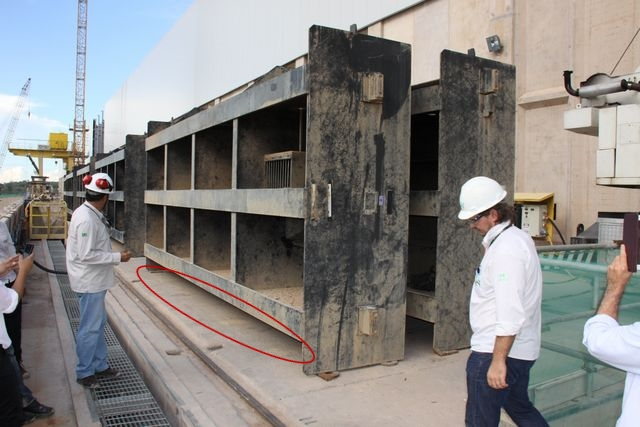
\includegraphics[width=0.6\columnwidth]{figs/op_rem_3_1}
    \caption{Equipe conhecendo a montagem de turbinas.}
    \label{fig:op_rem_3_1}
\end{figure}

O experimento visa, então, adquirir uma base de
dados para que se possa identificar as propriedades específicas do ambiente a ser inspecionado e, assim, 
elaborar estratégias para a eliminação, ou atenuação dos ruídos presentes no
ambiente e, também intrinsecos do próprio sonar.

O experimento constituiu, primeiramente, na avaliação na melhor posição
para a fixação do sonar à viga utilizando a estrutura metálica desenvolvida em
laboratório pelo Prof. Ramon, visando um maior aproveitamento do ponto de vista
e uma menor quantidade de ruídos referentes á posição. O projeto mecânico foi
desenvolido a partir do desenho detalhado da viga, disponível em CAD.

O sonar é alimentado por duas baterias de $12V$, $7Ah$, em série, formando uma
alimentação de $24V$. A potência é transmida ao sensor por meio do cabo
umbilical, que também é responsável pela comunicação de dados entre o sonar e o
computador em terra.

Os resultados deste experimento mostraram que a configuração da estrutura do
%TODO verificar nomes 
poço/fosso e o ambiente adjacente (turbinas em funcionamento, correnteza do rio
e turbilhamento) não interferem de forma que impossibilite o desenvolvimento de
um sistema de reconstrução 3D do fundo do rio para a operação de inspeção do
mesmo.
